%* what is known
Localized surface plasmon resonance (LSPR) is an optical effect where the electronic
cloud around a metallic nanoparticle resonates with an incoming electromagnetic 
field (see Figure \ref{fig:lspr}). When this happens, most of the incoming wave 
is either absorbed by the nanoparticle, or scattered in different directions,
generating a large shadow behind the scatterer. This principle is used to design 
biosensors, as the resonance frequency shifts when analytes bind to the metallic
nanoparticle \cite{HaesETal2004, HaesVanduyne2002}, resulting in highly sensitive sensors.

In the LSPR application, numerical simulations are scarsely used, and they rely on the 
solution of Maxwell's equations in some form. These simulations have been used to study the 
optical properties of dielectric or metallic nanoparticles \cite{Hohenester2018,
JungPedersenSondergaardPedersenLarsenNielsen2010, VideenSun2003,
MayergoyzFredkinZhang2005, MayergoyzZhang2007}, interactions between nanoparticles
and electron beams \cite{GarciadeabajoAizpurua1997, GarciadeabajoHowie2002},
surface plasmon resonance sensors \cite{JungCampbellChinowskyMarYee1998} and
biosensors \cite{HaesETal2004, HaesVanduyne2002} interaction of molecules and
localized surface plasmons in metallic particles \cite{DavisGomezVernon2010,
AntosiewiczApellClaudioKall2011}. Among the methods used in these simulations 
we find finite difference time-domain (FDTD) and boundary elements\cite{Garciadeabajo}.

{\color{red} Not sure how to talk about the different methods, any idea? should
we talk about this? 

Methods: fem (comsol), fdtd (davis and coworker), bem (garcia de abajo and 
howie, bem ++, matlab guy). van duyne and haes? }
{\color{blue} wrote something there, let me know what you think. My impression is that
we shouldnt talk too much on this.}

Localized surface plasmon resonace is an optical effect that is involved in the
design of certain nanosensors due to their high sensitivity. LSPR is an 
optical phenomenon that ocurrs when light shines on conductive nanoparticles
that are smaller than the wavelength of the incident light. The free electrons
on the surface of the nanoparticle are excited by the incoming electric field
oscillating with it and creating plasmons. See Figure \ref{fig:lspr}

\begin{figure}[h] %  figure placement: here, top, bottom, or page
   \centering
   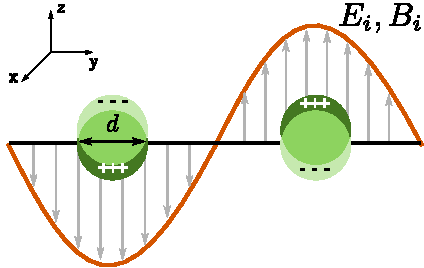
\includegraphics[width=0.35\textwidth]{lspr.pdf} 
   \caption{Localized Surface Plasmon Resonance (LSPR) scheme. }
   \label{fig:lspr}
\end{figure}

When plasmons resonate with the incoming electric field we end up with high 
levels of extinction, which is absorption plus scattering. LSPR biosensors are 
based on this effect and use the fact that this behaviour is highly dependant
on the dielectric of the local environment, resulting in a shift in the 
resonance frequency as the analyte approaches the nanoparticle.  

%* What is unkown, limitations and gaps

In the biosensor's community most findings and desicions in designed are achived 
through experimental analyses, trial and error procedures. Using software to 
assit the design and manufacturing process can play a key role for the future
of biosensors. In particular, experiments suggest that the distance between the
nanoparticle and the analyte affects the sensitivity of the sensor
\cite{HaesETal2004}. However, the processes to lead to this conclusions, were 
trial an error processes. Therefore, there is not enough understanding on what 
is the relation between high dependance on sensitivity on distance in 
biosensors, specifically LSPR biosensors.Most of the softwares that are used to 
approach this phenomenon use models of 
the nanoparticle and the analyte that are extremely simplistic. Moreover, the 
lack of grid convergence analysis and error study in most of the softwares in 
the plasmonic community, {\color{red}(I haven't find any of this in 
their papers, Chris what do you know about BEM++)} force the user to believe 
in the obtained results without knowing their uncertainty.

%* Fill the gap

Even though LSPR is an optical effect see Figure \ref{fig:lspr}, electrostatics 
makes a good approximation in the long-wavelength limit. In this work we use
\pygbe to study how the LSPR response changes in the presence
of a biomolecule. \pygbe most recent application \cite{ClementiETal2017} aims 
to guide the reasearch process in the design of biosensors. We treat localized 
surface plasmon resonance (LSPR) quasi-statically \cite{MayergoyzZhang2007} and
using an accurate representation of the biomolecule obtained thorugh the 
crystal structure from the protein data bank. To our knowledge, \pygbe is the 
only open-source software that uses a Tree code fast algorithm—O(N logN), for 
N unknowns, GMRES iterative solver; and hardware acceleration on GPUs to compute
the extinction cross-sections of arbitrary geometries. The software
\footnote{\url{https://github.com/barbagroup/pygbe}} is shared under the 
BSD 3-clause license and the development repository is available on Github.

{\color{red}  Keeping this structure here for reference until we polish better
the introduction.

What is known:
\begin{itemize}
\item Plasmonic simulations, what applications they cover, etc. (cite Matlab guy, also Garcia de Abajo, Jung+Pedersen, etc. Maybe we can even cite COMSOL here)
\item LSPR: how does it work, what simulations are there in the litarature. Talk about work from, for example, Davis or van Duyne. See page 50 of my thesis (end chapter 2).
\end{itemize}

What is unkown:
\begin{itemize}
\item all developments are trial and error
\item no computational tools to help in the design process
\item example: no understanding of the sensitivity of the system
\item models that consider the nanoparticle and the analyte are extremely simplistic
\end{itemize}

Fill the gap:
\begin{itemize}
\item design of a computational tool that is highly accurate to represent the biomolecule
\end{itemize}
}

